\chapter{Inteligência artificial}\label{cap:ia} % ou aprendizado de máquina?
\section{Introdução}\label{sec:ia_intro}
A inteligência artificial é um amplo ramo que trata de sistemas capazes de aprender e interpretar informações, e usar esse aprendizado para objetivos específicos.
%TODO: citação haenlein
Um dos campos da inteligência artificial é o aprendizado de máquina, onde a unidade de computação aprende a performar uma tarefa a partir de um conjuntos de exemplos de treinamento,
%TODO: citação louridas
funcionando como um tipo de modelo computacional do cérebro. Esses modelos são construídos a partir da interconexão entre unidades de processamento, por vezes chamados de neurônios artificiais, e por isso são conhecidas como \textbf{redes neurais artificiais}.

O tipo mais comum de aprendizado de máquina é o chamado \textbf{aprendizado supervisionado}, onde o modelo é apresentado a um conjunto de dados de exemplo que são rotulados, ou seja, cada entrada tem a sua saída definida. Durante o aprendizado, o modelo fornece uma saída e, a partir da saída verdadeira, ele se ajusta internamente para se aproximar mais do real.
%TODO: citação lecun
Quando não há uma saída real rotulada disponível, pode-se utilizar o \textbf{aprendizado não-supervisionado}. Nesse caso, o modelo tenta aprender alguns padrões nos dados, como grupos de exemplos similares. O aprendizado não-supervisionado tem a capacidade de identificar novos tipos de informações, já que não estão restritos aos rótulos.
%TODO: citacao aniscar

Os algoritmos de aprendizado de máquina também podem ser divididos quanto à atividade a ser realizada. Atividades de \textbf{classificação} identificam a classe da informação (por exemplo, se um animal é um cão ou gato) a partir de dados rotulados, o \textbf{agrupamento} (\textit{clustering}, em inglês) determina classes agrupando informações similares em grupos (\textit{clusters}) rotulados (como o agrupamento de filmes em gêneros), a \textbf{regressão} é usada para prever algum valor ou quantidade (como o preço de ações ao longo do tempo), e a \textbf{redução de dimensionalidade} representa dados de várias dimensões em outras menores (como as várias informações de um paciente sendo reduzidas às mais importantes para o diagnóstico de uma doença).

\section{Redes neurais}\label{sec:redesneurais}
O primeiro modelo de neurônio artificial foi o de McCulloch-Pitts, baseado em lógica binária e que possuía duas fase, a primeira onde o neurônio soma as contribuições de todos os neurônios anteriores, e a segunda onde o neurônio dispara apenas se um limiar for ultrapassado e não houver disparo de neurônio inibitório.
%TODO: citação mcculloch
Apesar de revolucionário para a época, um dos principais problemas do modelo de McCulloch-Pitts era a ausência do ajuste de pesos, ou seja, as conexões entre os neurônios sempre tinham a mesma força. Muitas pesquisas se desenvolveram na área para suprir essa necessidade, até que Frank Rosenblatt, inspirado pela teoria de Hebb vista anteriormente, criou o \textit{Perceptron},
%TODO: citacao rosenblatt
desenvolvido para ser um neurônio mais generalizado, sendo a base do aprendizado de máquina moderno. Matematicamente, o \textit{Perceptron} pode ser modelado pela seguinte equação:
\begin{equation}\label{eq:perceptron}
	y=\sigma\Big(\sum_{k=1}^Nw_kx_k+b\Big)
\end{equation}
onde $x_k$ é a resposta da sinapse $k$, $w_k$ é o peso da sinapse, $b$ é o \textit{bias} (viés, em português), um peso de referência que representa um conhecimento a priori, %TODO: elaborar
$\sigma$ é uma função de ativação não-linear, e $y$ é a saída do neurônio, como representado na Figura~\ref{fig:perceptron}. Resolvido o problema da atualização dos pesos, o \textit{Perceptron} sozinho é incapaz de realizar tarefas de separação não-linear,
%TODO: citação minsky
levando à criação, muitos anos depois, do \textit{Perceptron} de multi-camadas (MLP, \textit{Multilayer perceptron}, em inglês), que supre as limitações do \textit{Perceptron} simples ao agrupar camadas de neurônios, como na Figura~\ref{fig:mlp}. As camadas presentes entre a entrada e a saída da rede são chamadas de camadas ocultas (ou intermediárias).
\begin{figure}
	\centering
	\caption{Arquiteturas do Perceptron}
	\label{fig:perceptrons}
	\begin{subfigure}[b]{0.3\textwidth}
		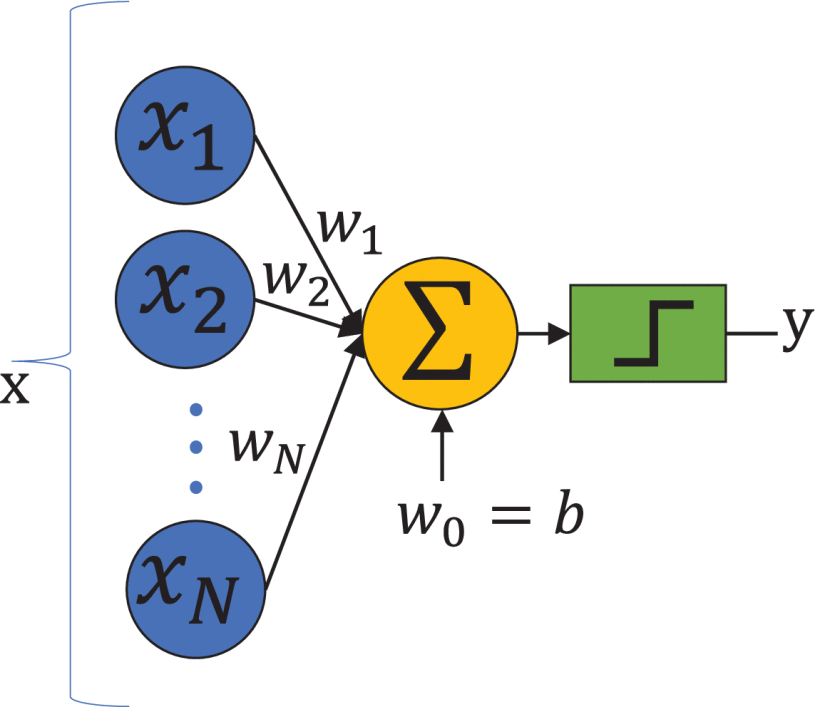
\includegraphics[width=\textwidth]{figs/perceptron}
		\caption{Perceptron}
		\label{fig:perceptron}
	\end{subfigure}
	\qquad\qquad
	\begin{subfigure}[b]{0.3\textwidth}
		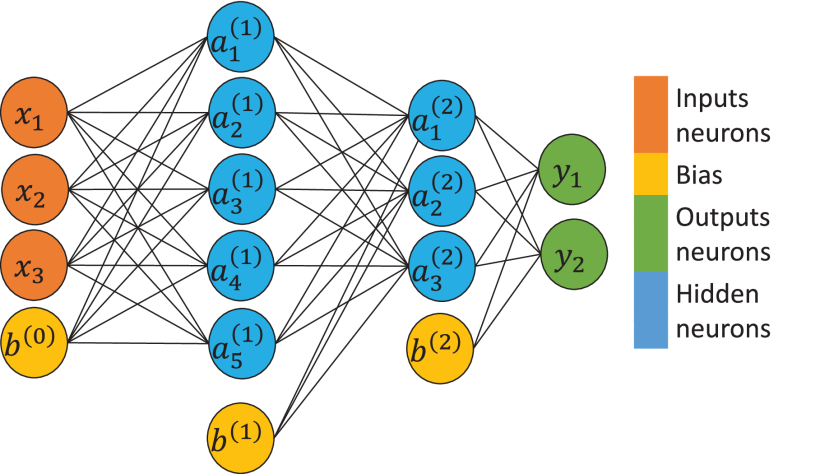
\includegraphics[width=\textwidth]{figs/mlp}
		\caption{Perceptron de multi-camadas}
		\label{fig:mlp}
	\end{subfigure}
\end{figure}

Os vários neurônios presentes nessa arquitetura frequentemente têm seus pesos atualizados através do algoritmo de gradiente descendente, que busca minimizar o erro entre a saída obtida pela rede e a real (aprendizado supervisionado), e essa atualização é feita através da metodologia da retro-propagação (\textit{backpropagation}, em inglês), ou seja, as atualizações das camadas finais da rede são propagadas em direção às iniciais.
%TODO: citação werbos
Quando há uma grande quantidade de camadas na rede ela é chamada de rede neural profunda (\textit{deep neural network}, em inglês), permitindo um mapeamento de dados mais complexos, o que não seria muito eficiente em redes não profundas. Uma lista não exaustiva de arquiteturas, profundas ou não, é apresentada abaixo:
\begin{alineas}
	\item \textbf{\textit{Convolutional Neural Networks} (CNN, Redes neurais convolucionais)}: possui camadas que implementam a operação matemática de convolução, aplicando um filtro no sinal, e camadas de sub-amostragem (\textit{downsampling}), chamadas de \textit{pooling}. Essas redes lidam bem com sinais em duas dimensões, e por isso são frequentemente aplicadas em tarefas de visão computacional (relacionadas a imagens e vídeos);
	%TODO: citação lecun gradiente
	\item \textbf{\textit{Recurrent Neural Networks} (RNN, Redes neurais recorrentes)}: muito usadas em tarefas de entradas sequenciais, como processamento de fala e linguagem, possem a característica de processar os dados elemento a elemento, considerando também informações dos elementos passados, armazenados em pesos de conexões recorrentes, que funcionam como uma memória dinâmica para a rede;
	%TODO: citação elman finding
	\item \textbf{\textit{Hopfield Networks} (Redes Hopfield)}: proposta por J. J. Hopfield, são redes que são treinadas para aprender padrões (memórias) dos dados de maneira associativa, baseado no princípio de Hebb de que neurônios que disparam juntos se conectam;
	%TODO: citação hopfield
	\item \textbf{\textit{Autoencoder} (auto codificador)}: redes que aprendem a representar os dados reduzindo sua dimensionalidade, diminuindo as camadas ocultas, e, posteriormente, recriando os dados originais;
	%TODO: citação hinton reducing
	\item \textbf{\textit{Long Short-Term Memory} (LSTM)}: uma variação da RNN composta de 4~(quatro) blocos de memória, sendo um principal e os outros três, chamados de portões de entrada, esquecimento e saída, responsáveis por alterar o estado da célula como um todo.
	%TODO: citação hochreiter
	Devida à sua capacidade de reter informações de longo tempo em séries temporais, são muito usadas em sistemas de reconhecimento de voz;
	\item \textbf{\textit{Spiking Neural Networks} (SNN, redes neurais de disparo)} testando
\end{alineas}

% backprop/grad desc

% lstm

\section{Redes neuromórficas}\label{sec:redesneuromorficas}
% estado da arte
% hardware neuromórfico (von-neumann vs neuromorfico)

\begin{itemize}
	\item Redes neurais de disparo usam neurônios de disparo como unidades de computação, como os modelos \textit{Leaky integrate-and-fire} (LIF) e o modelo de Izhikevich
	\item As unidades de computação são conectadas entre si e interagem através das sinapses (Figura~\ref{fig:sinapse})
\end{itemize}

\begin{figure}[htb!]
	\centering
	\caption[Neurônios pré e pós sinápticos conectados através de uma sinapse]{Neurônios pré (verde) e pós (roxo) sinápticos conectados através de uma sinapse. Os neurotransmissores (círculos vermelhos) são liberados do axônio pré-sinaptico para o dendrito pós-saptico, gerando potenciais pós-sinapticos que podem ser excitatórios (EPSP) ou inibitórios (IPSP). No neurônios pós-sinaptico os potenciais de todos os dendritos são somados e, dependendo do valor total, um potencial de ação (AP) pode ser gerado}
	\label{fig:sinapse}
	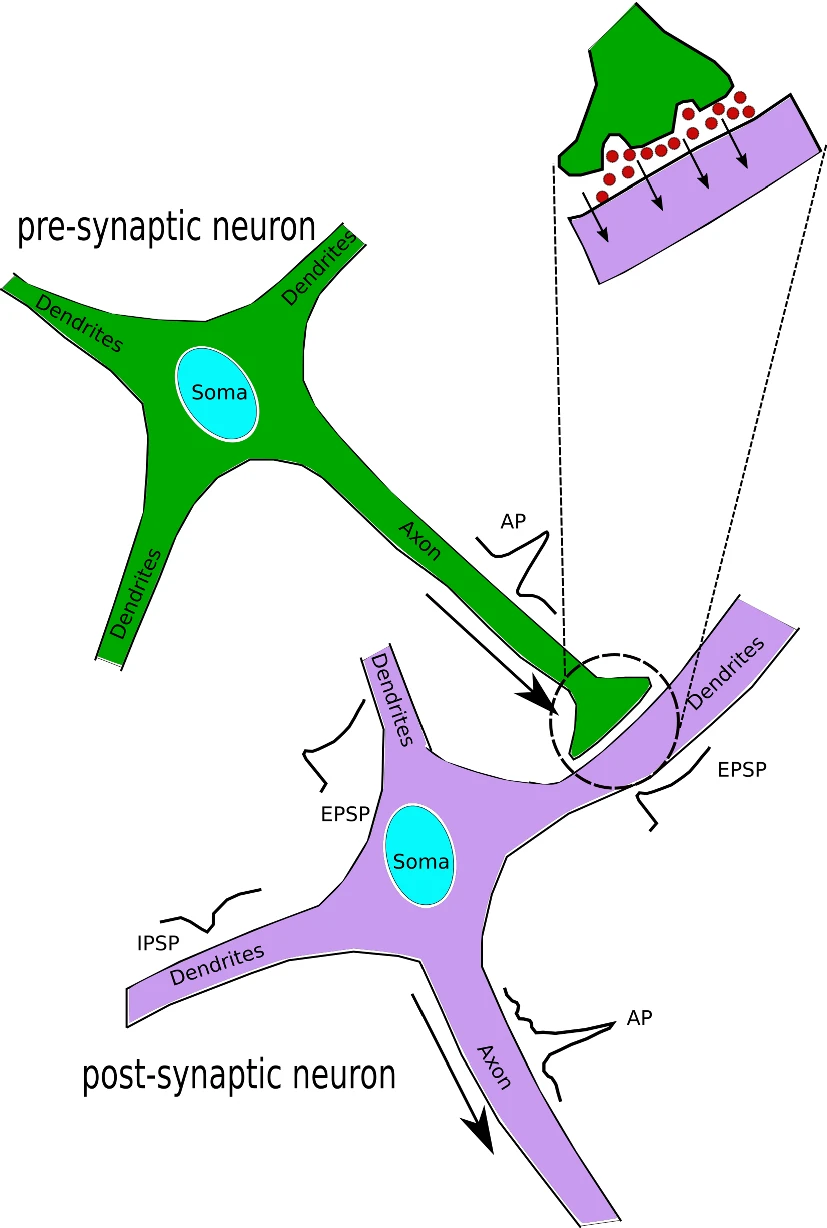
\includegraphics[width=0.3\linewidth]{figs/sinapse}
\end{figure}

\subsection{Processamento de informação}
\begin{itemize}
	\item A informação recebida pelas redes precisa ser codificada, e dois métodos para isso são:
	\begin{description}
		\item[Codificação de taxa] A taxa de disparo dos neurônios é usada. A taxa pode ser calculada como a média temporal (quantidade de disparos por intervalo de tempo), média de disparos em \textit{trials} diferentes, dentre outras maneiras
		\item[Codificação de tempo de disparo] O instante exato de ocorrência de disparos individuais é usado. Dentre os tipos de codificação nesse caso incluem-se o tempo do primeiro disparo (o tempo entre o início do estímulo e a ocorrência do primeiro disparo), a codificação de ordem (a ordem em que os neurônios disparam é o código), a codificação de latência (a diferença de tempo entre os disparos), dentre outras
	\end{description}
	\item Os critérios para seleção do método de codificação variam por diferentes aspectos, como a \textbf{minimização da perda de informação após a decodificação} e o \textbf{aumento da acurácia de previsão/classificação}
\end{itemize}

\subsection{Aprendizado das redes de disparo}
\begin{itemize}
	\item Para cada tipo de codificação citada acima, um método de aprendizado é empregado, que são:
	\begin{description}
		\item[Aprendizado baseado em taxa] Uma variação do método \textit{backpropagation} é usada aqui, relacionando as ativações das unidades das redes neurais com as taxas de disparo
		\item[Aprendizado baseado em disparo] Utiliza a plasticidade dependente de tempo de disparo (STDP, \textit{spike-timing dependent plasticity}),onde os pesos das conexões sinapticas são proporcionais ao grau de relação entre os tempos de disparo pré e pós-sinapticos (Figura~\ref{fig:stdp})
	\end{description}
\end{itemize}

\begin{figure}[htb!]
	\centering
	\caption{Conceito da STDP}
	\label{fig:stdp}
	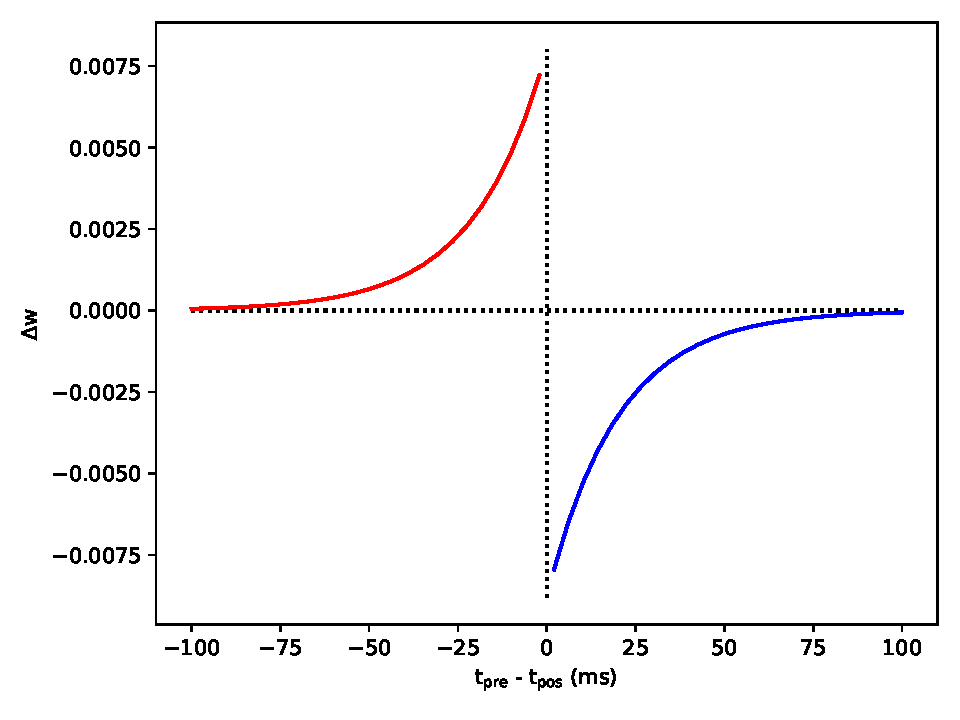
\includegraphics[width=0.7\linewidth]{figs/stdp}
\end{figure}



% pensar onde colocar os simuladores
% \section{Simuladores neuronais}\label{sec:simuladores}
